\labday{20 March 2023}

\experiment{PPDr}

PPD is no longer functional after returning from a campaign in northern Finland. There are no useful images on the screen. When the trigger threshold is lowered to 10, and the trigger PMT voltage is raised above 20, there are noise triggers.

PPD was removed from its pelicase, removing and breaking the seal of the 4 bolts. The inlet heaters were disconnected, and the pump was removed. The arduino was reprogrammed to not trigger the relays. PPD was suspended above  the pelicase on two poles. The grounding point was replaced and connected to the mains socket, the mains cable was also replaced with an English plug.

There was water in the tube of the bleed flow, it is suspected that this is what damaged the pump, therefore meaning that the water trap does not work properly. The water is shown in Fig. \ref{fig:PPDWaterTube}.

\begin{figure}[H]
\begin{center}
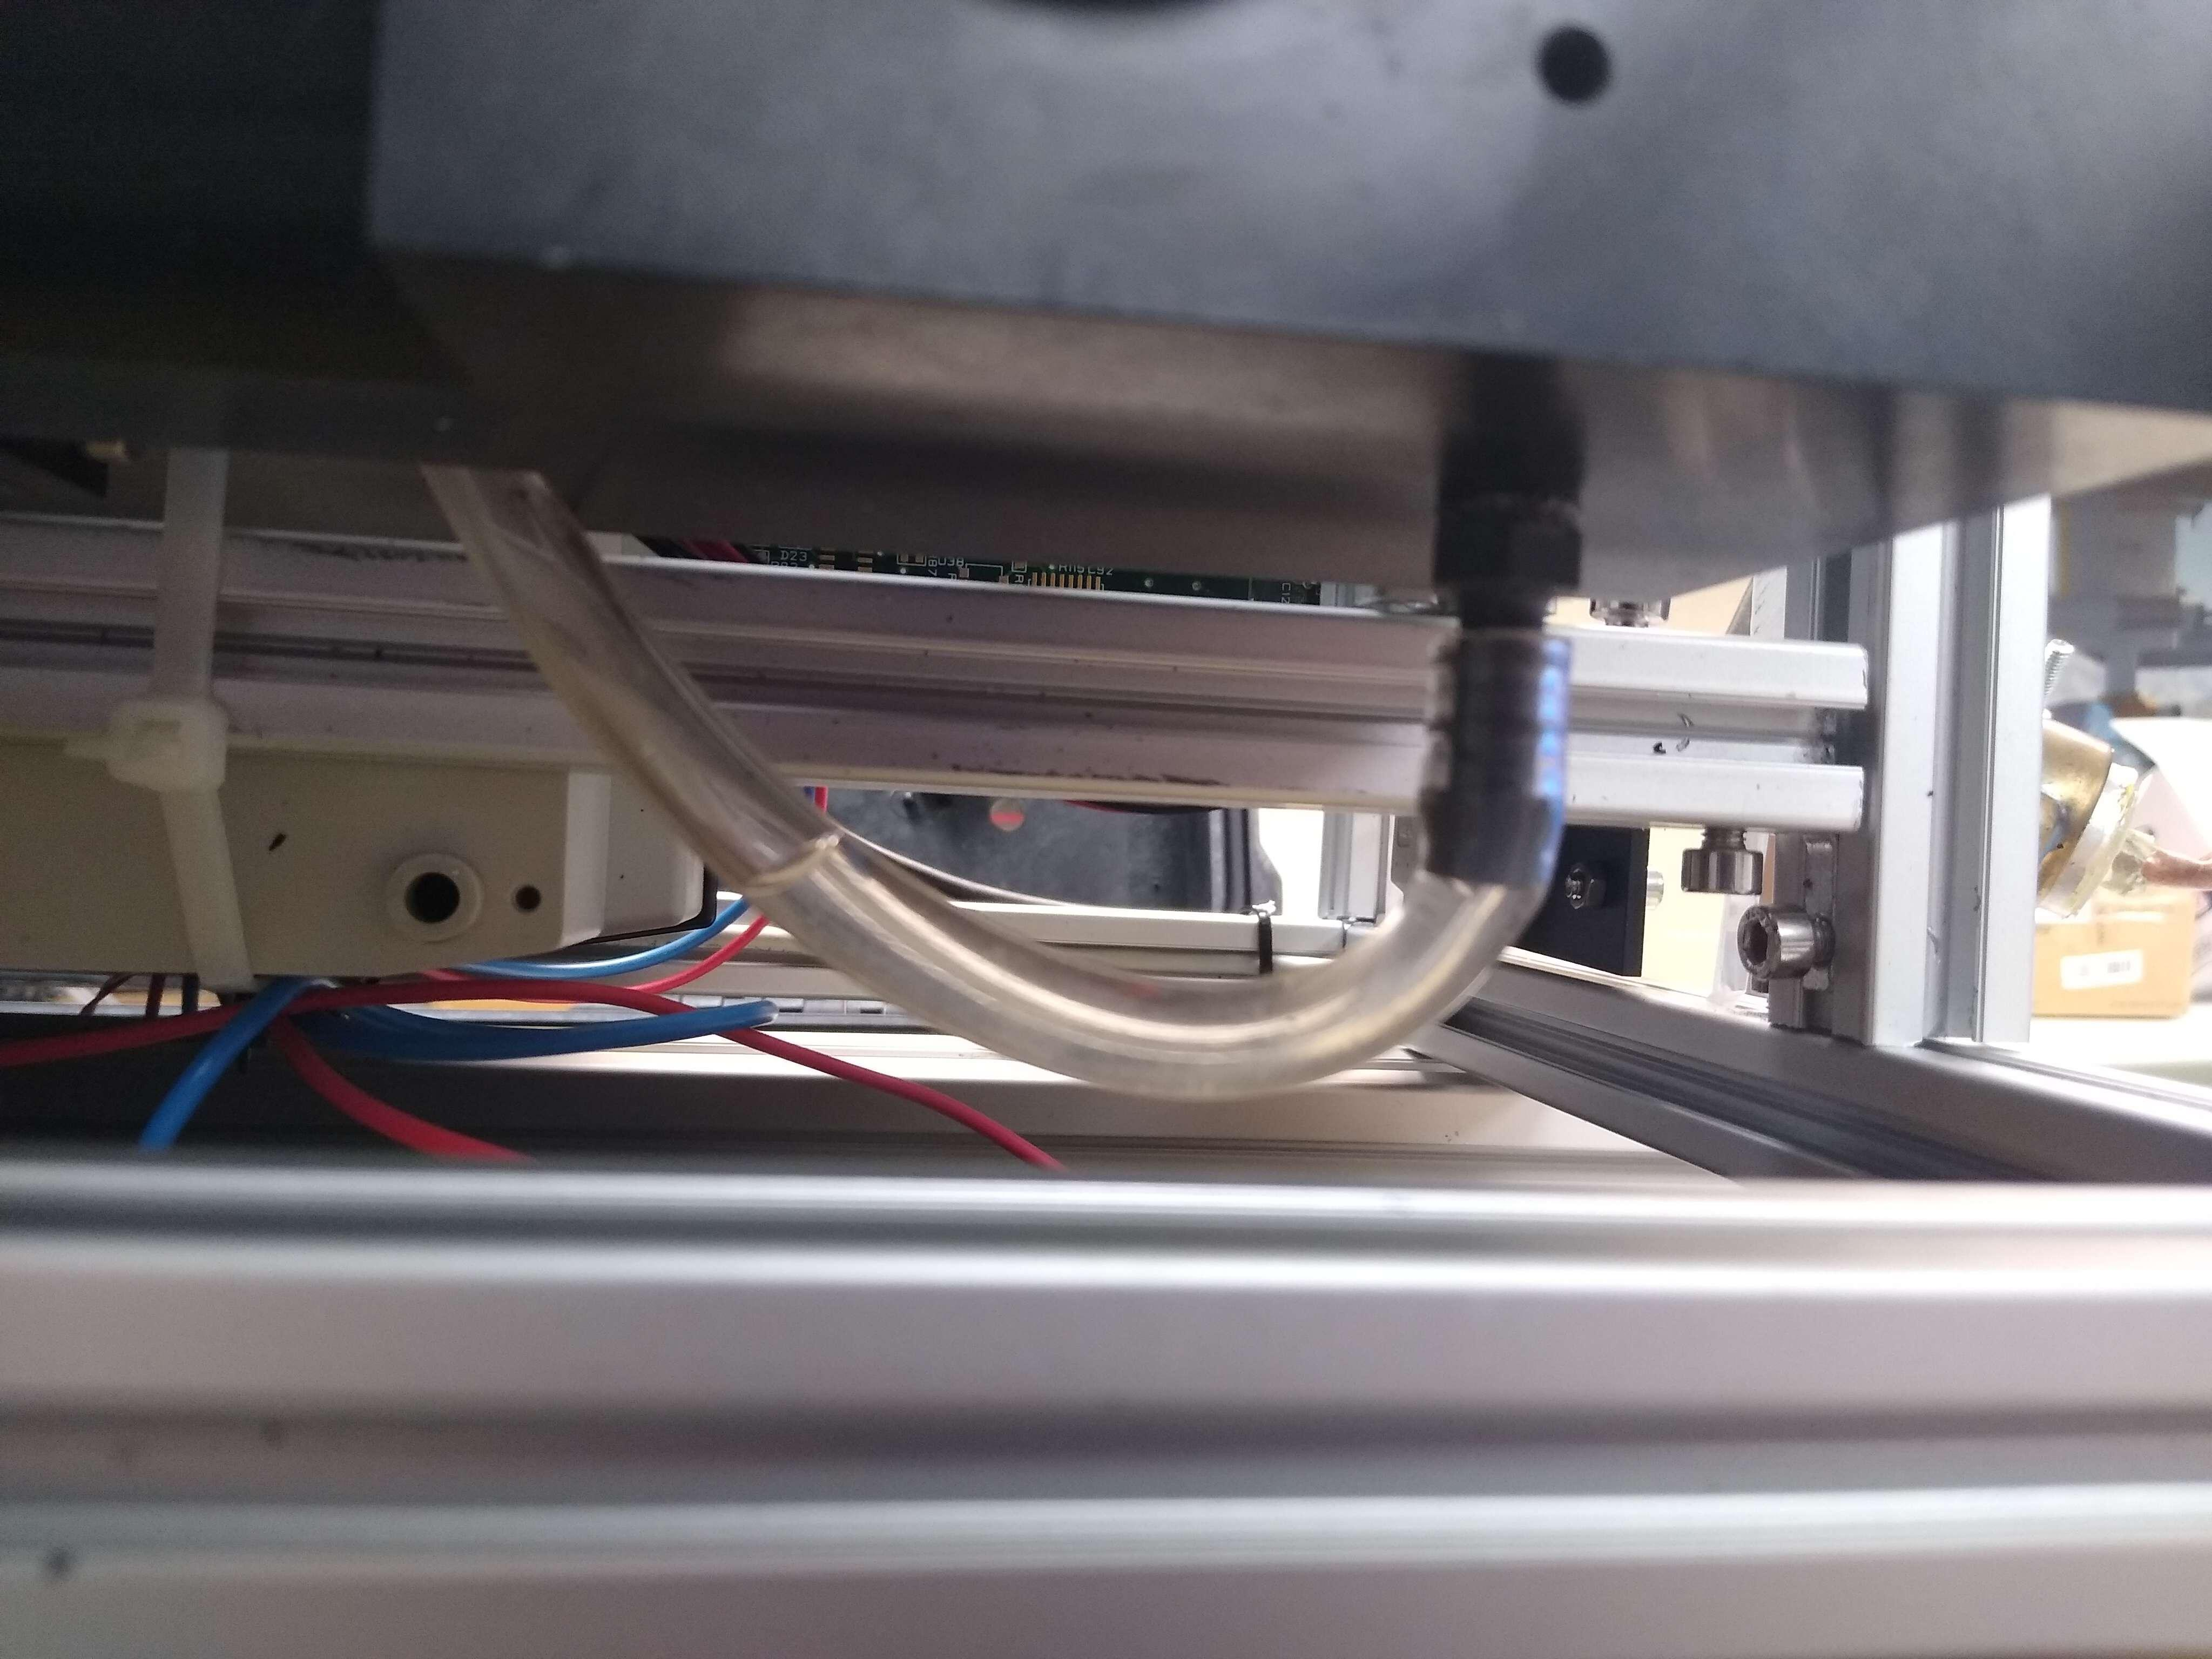
\includegraphics[width=0.5\linewidth]{Figures/PPDWaterTube}
\end{center}
\caption{Water in bleed tube.}
\label{fig:PPDWaterTube}
\end{figure}

There was also a white deposit on the inside of the inlet. Upon examination with the endoscope, it was review that this deposit did not settle on the lens system. This is shown in Fig. ref{PPDInletDeposit}

\begin{figure}[H]
\begin{center}
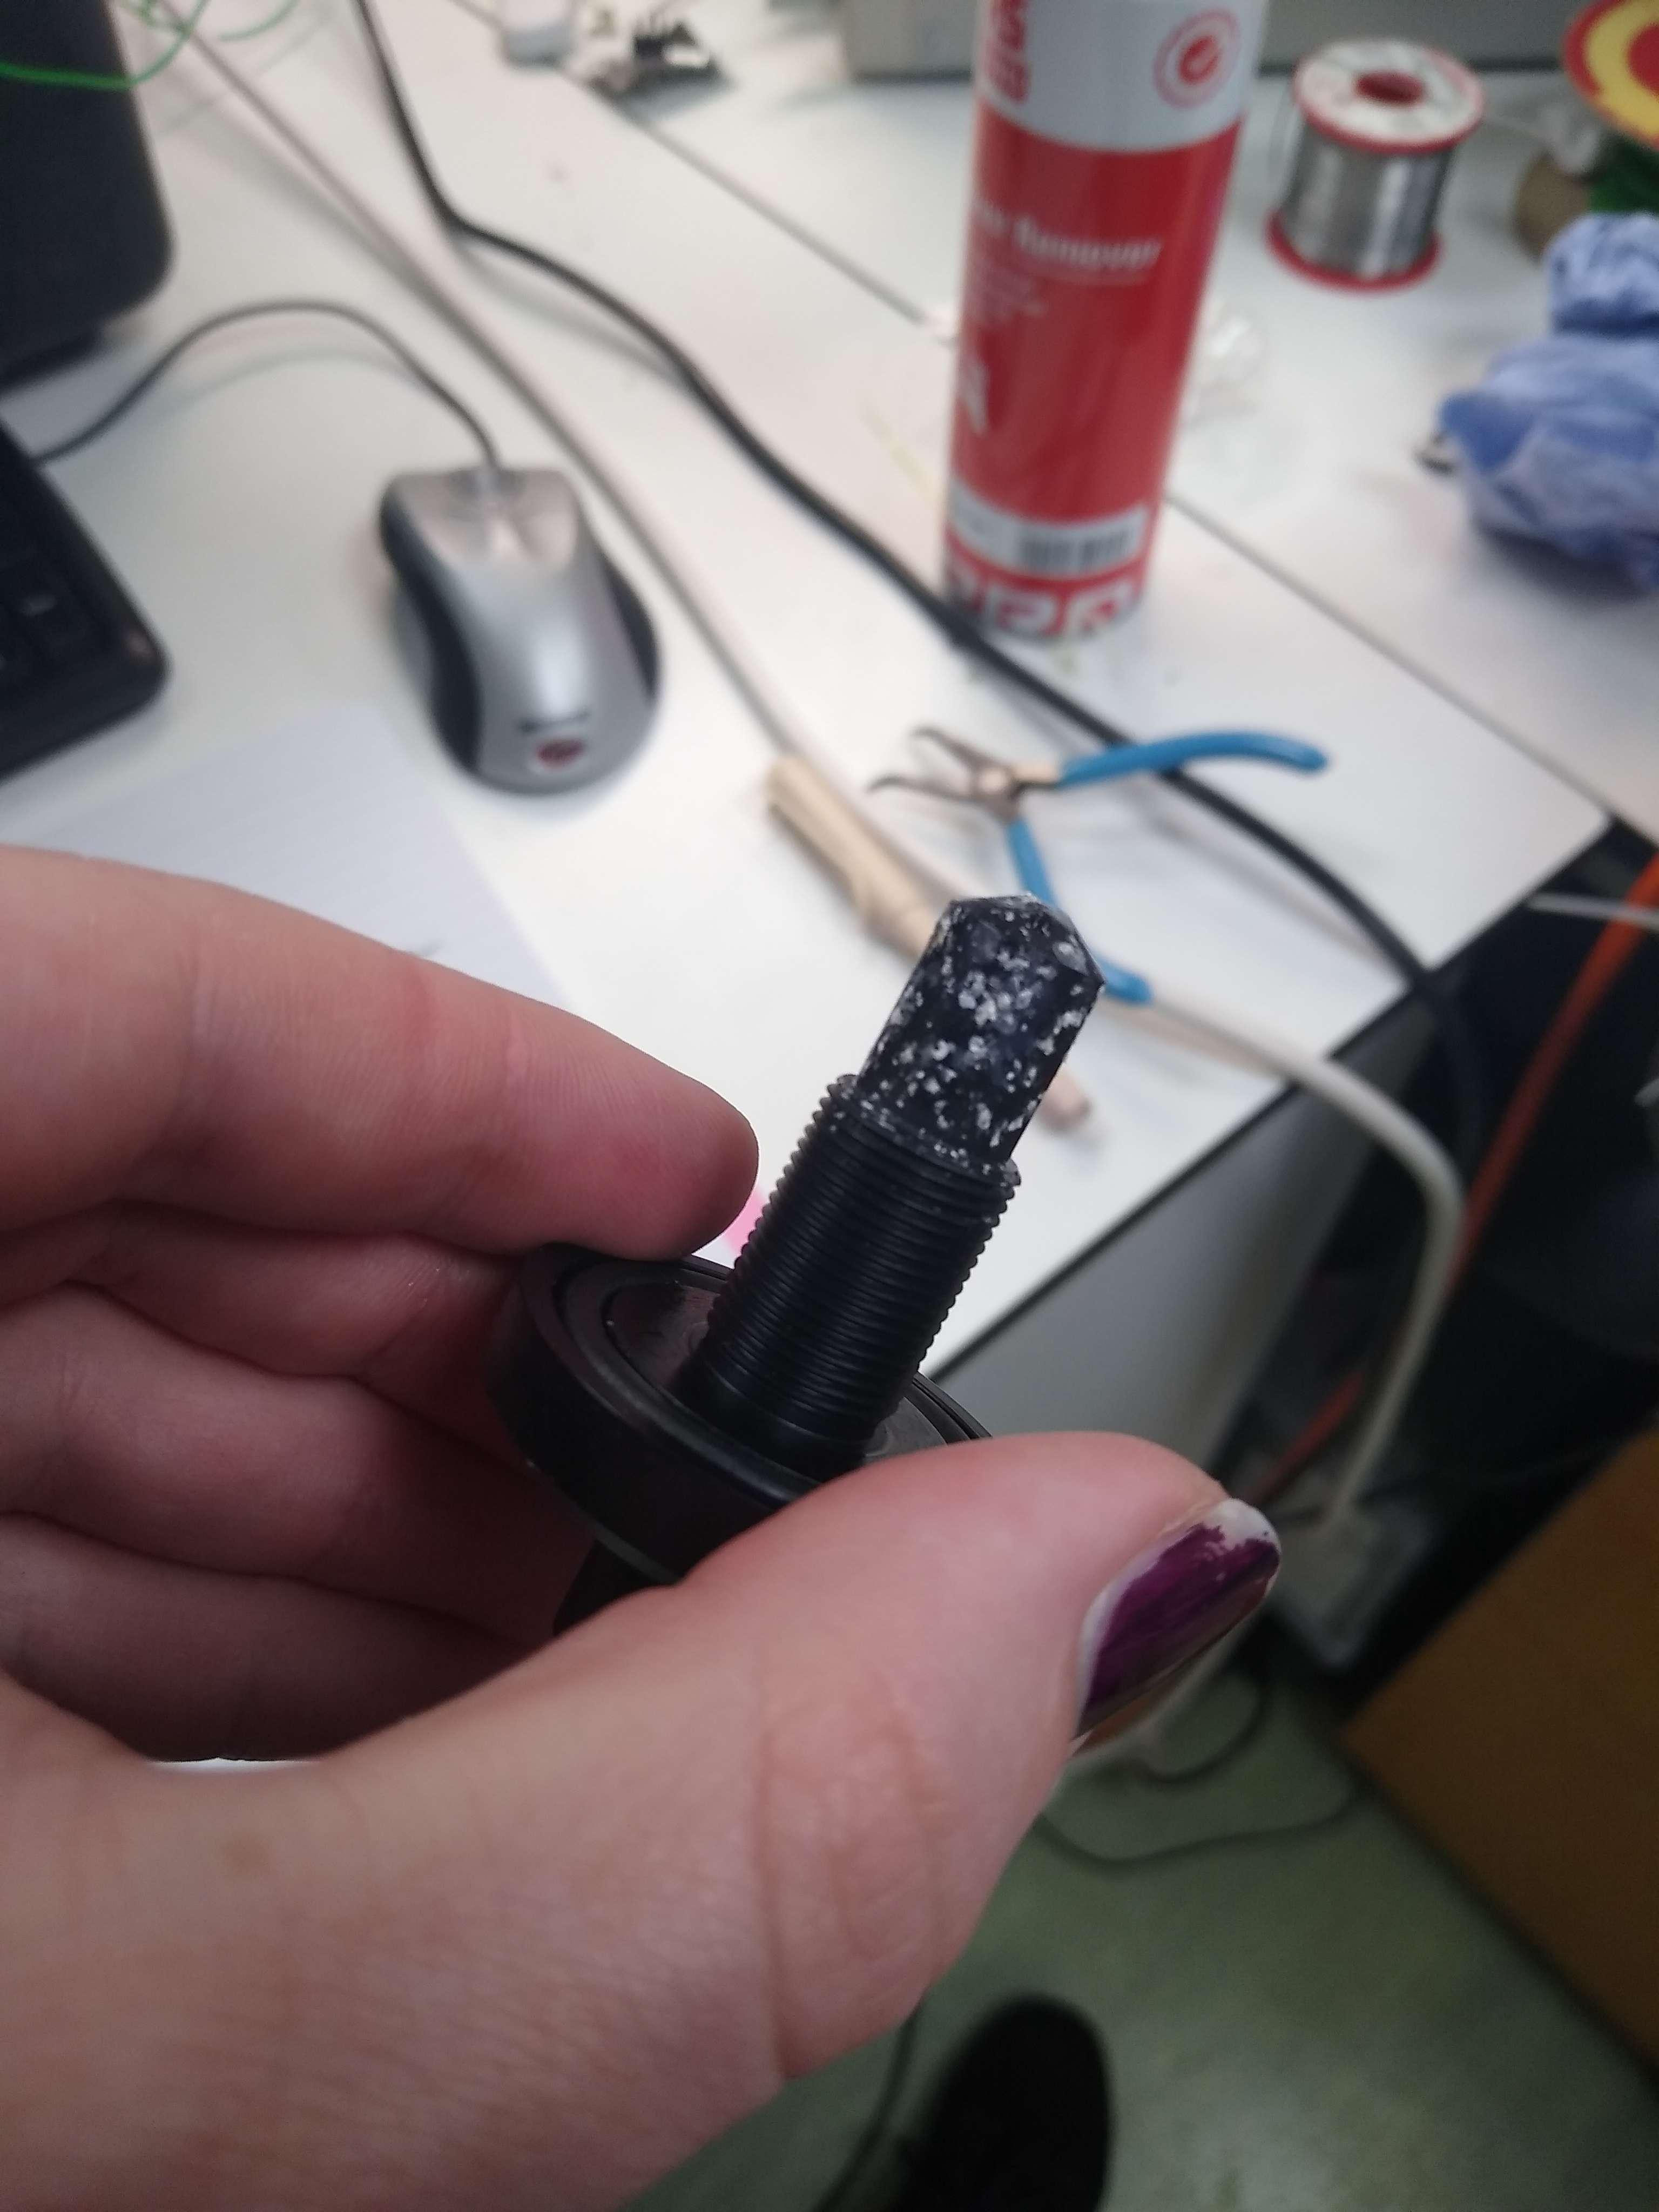
\includegraphics[width=0.5\linewidth]{Figures/PPDInletDeposit}
\end{center}
\caption{Deposit on PPD inlet.}
\label{fig:PPDInletDeposit}
\end{figure}

Once the inlet was removed, the scattering off large objects could be faintly observed. Adjusting the camera gain to maximum led to shot noise, and did not improve the image much. The scattering can be seen in Fig. \ref{fig:PPDPenScatter}

\begin{figure}[H]
\begin{center}
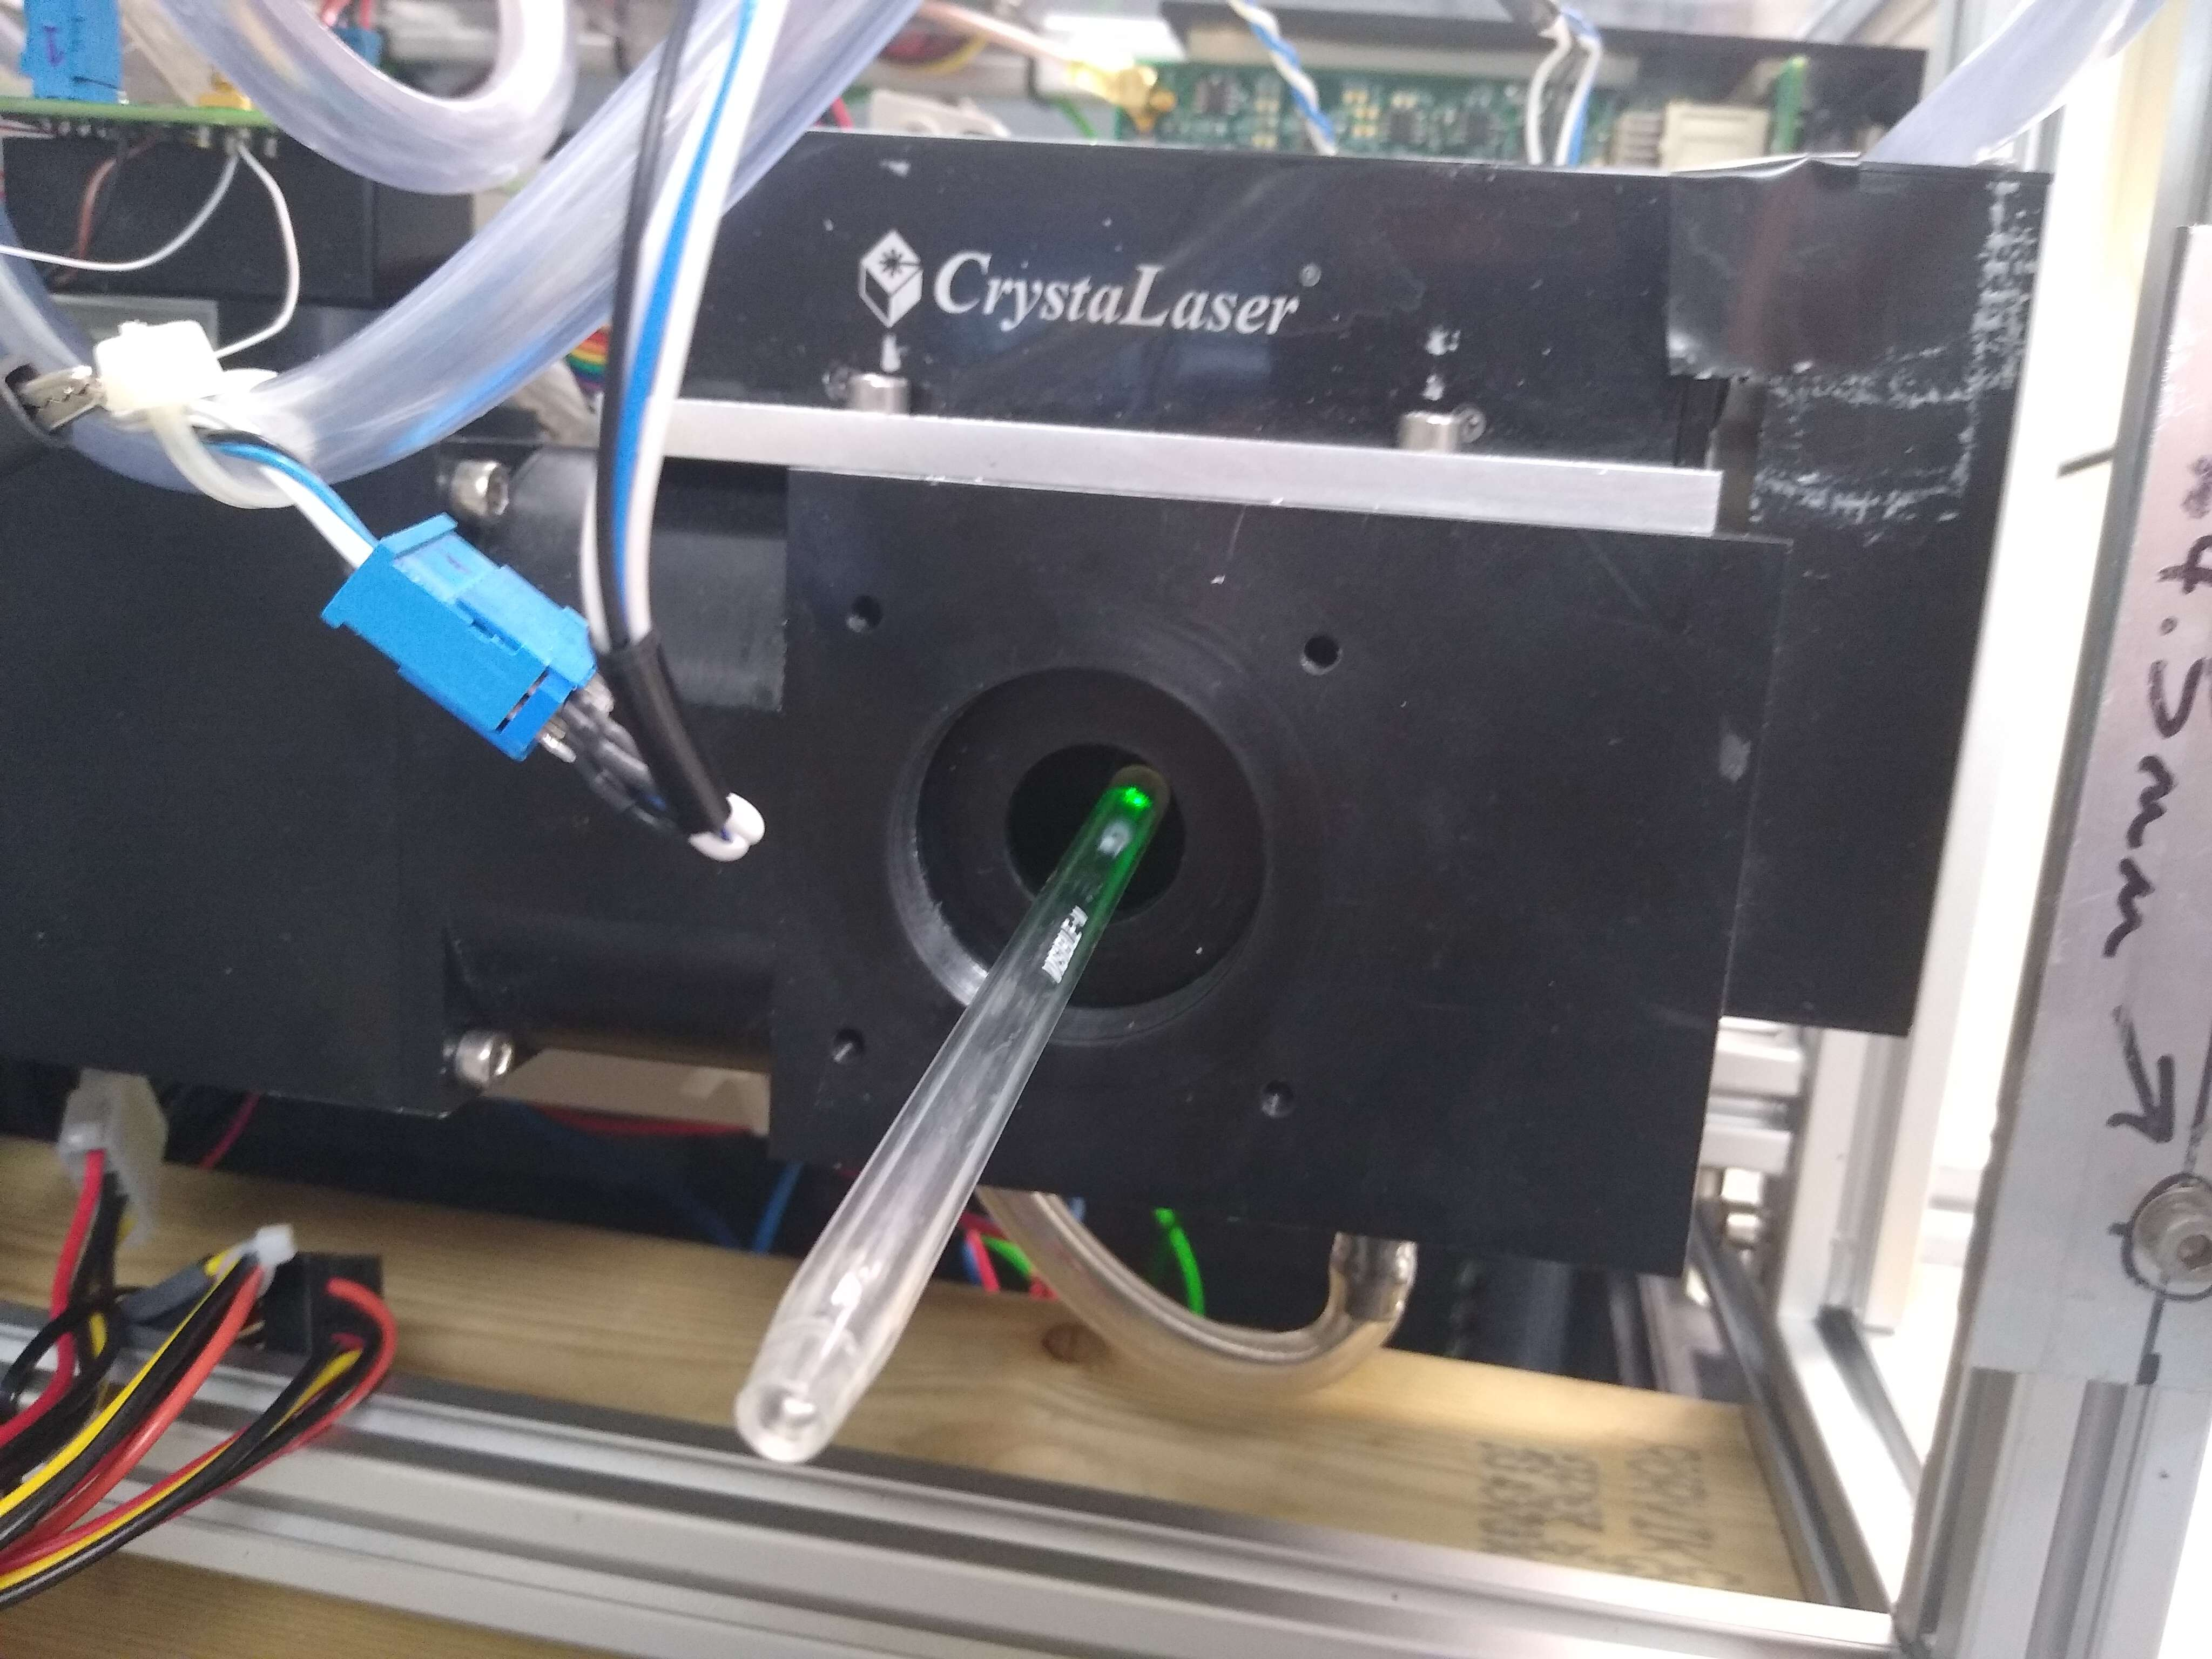
\includegraphics[width=0.5\linewidth]{Figures/PPDPenScatter}
\end{center}
\caption{Scattering off pen.}
\label{fig:PPDPenScatter}
\end{figure}
